%%%%%%%%%%%%%%%%%%%%%%%%%%%%%%%%%%%%%%%%%%%%%%%%%%%%%%%%%%%%%%%%%%%%%%%%%%%%%%%%
% experiment.tex: Chapter describing the experiment
%%%%%%%%%%%%%%%%%%%%%%%%%%%%%%%%%%%%%%%%%%%%%%%%%%%%%%%%%%%%%%%%%%%%%%%%%%%%%%%%
\chapter{Hadron Collider and Detector}
This section describes the particle collider and detector. The first section describes the particle accelerator which is the Large Hadron Collider~(LHC) and the next section describes the Compact Muon Solenoid~(CMS) detector with emphasis to those sections directly relevant to this analysis. A detailed description of the LHC and CMS detector is found in \cite{LHC} and \cite{CMSTDR}.
\section{Large Hadron Collider}
\subsection{Overview}
The LHC is a proton-proton and heavy ion collider designed to achieve a center of mass $\displaystyle{\sqrt{S}}$ energy of 14~TeV. It is hosted by the European Organisation for Nuclear Research~(CERN). Unlike linear colliders, the LHC is a circular collider with nearly 27~km in circumference located at the border between France and Switzerland. It is designed to smash protons and ions against each other controlled by powerful magnets at four main points. The Compact Muon Solenoid~(CMS) is one of the multi-purpose particle detectors at each collision point.
%ranging from A Toroidal LHC Apparatus~(ATLAS) and
%both non-fixed target detectors, A Large Ion Collider Experiment~(ALICE) for colliding heavy ions and finally Large Hadron Collider beauty~(LHCb), a fixed target experiment for investigating the properties of B-Hadrons.
% We  give a full description of the important parts of the LHC in the following subsections, detail discussion of other interesting parts can be found here \cite{LHC}.
%There are three main steps prior to colliding protons or ions at the LHC.  The first is ramping up the energy of the beams followed by squeezing the beams at interaction points( CMS or ATLAS) and finally remove the separator bumps that are formed by local corrector magnets.
Fig. \ref{fig:LHC} shows the LHC and the different stages before particle collision.%Thus our description of the LHC will follow this three stages.
\begin{center}
\centering
\mbox{
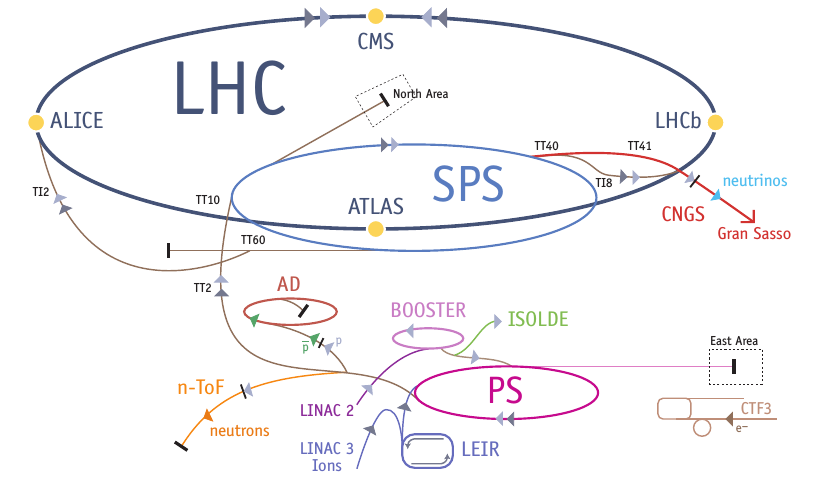
\includegraphics[width=6in]{THESISPLOTS/The_LHC.png}}
\captionof{figure}{Schematic diagram showing the full Large hadron Collider.} %Image taken from \cite{LHCB}}
\label{fig:LHC}
\end{center}
\subsection{Colliding Energy}
Hydrogen ions also known as protons from hydrogen gass where the orbiting electron has been striped away is inserted into a linear 
accelerator called \textit{Linac 2}.
Using electromagnetic fields in Radio Frequency~(RF) cavities, these protons are accelerated to an energy of 50~\MeV creating a stream of particles called \textit{particle beams} arranged in packets known as \textit{bunches}.
Protons from the Linac2 are injected into the circular synchrotron Booster~(PSB).
% The protons surf this electromagnetic fields and are group in troughs of the electromagnetic waves called RF~\textit{buckets}.
The circular synchrotron accelerator ensures that the protons pass many times through a cavity with their energy slowly increasing each time to reach the design energy.
The PSB accelerates the protons up to 1.4~\GeV and inject them into the Proton Synchrotron~(PS) which increases their energy to 25~\GeV. These protons traveling at 99.93\% the speed of light are sent to the Super Proton Synchrotron~(SPS) and accelerated to an energy of 450~\GeV. They are finally transferred into the LHC ring(accelerating in a clockwise and anti-clockwise direction) and accelerated for about 20 minutes to their nominal energy of 7~\TeV.By now the protons are traveling with the speed of 99.9999\% the speed of light.
Powerful bending magnets are used to keep the beams traveling in the circular LHC ring. The advantage of circular particle colliders  over fix target is that, the energy available to make new particles called the \textit{center of mass}~(COM) energy, denoted as $\sqrt{S}$ is simply the sum of the energy of the two beams \ie $\sqrt{S} = \mathit{E}_{\mbox{beam1}} + \mathit{E}_{\mbox{beam2}}$ compared to $\sqrt{\mathit{E}_{\mbox{beam}}}$ for fix target experiments. For the LHC, each beam is designed to have energy of 7~\TeV 
making $\sqrt{S} = 14$~\TeV. In circular colliders, synchrotron radiation~(is inversely proportional to the mass of the charge particle to the fourth power) by an accelerating charge particle contributing to loss its energy. This would require a continuous addition of energy after each turn to maintain the beam energy to a stable value. However, since the proton's mass is  about $0.938$~\GeV, and are to be accelerated to about $7$~\TeV, this loss of energy is not very significant unlike for electrons whose mass is about $0.000511$~\GeV and the energy loss is  more. Thus protons are preferred to electrons for a circular collider.
Then again, the debris of particles produced when electrons collide is much less compared to that of protons making analysis in a hadron collider very challenging. 
\subsection{Luminosity}
In colliding beams experiments, the center of mass energy available for the production of new effects is very important.
However, the number of useful interactions producing effects~(events) is equally important, especially
in cases where the probability~(also known as cross section,$\sigma$) of producing rare events is very small.
The quantity which measures the ability of a particle accelerator to produce the events from the required number of 
interactions is called \textit{luminosity}. The luminosity is also the proportionality factor between
the number of events per second and the cross section. Luminosity~($\mathscr{L}$) is therefore a measure of the number of collisions that can be produced in a collider per squared area per second. 
The cross section is calculated from theory while the luminosity depends on factors ranging from
the flux \ie number of particles per second  of the beams, the beam sizes at collision, and the frequency of collision.
For physics experiments, the integrated luminosity which is total luminosity over a given period of time
usually a year gives the amount of data that has been recorded by a given detector. 
%This is known as the instantaneous luminosity and it is related to the cross-section(a probabilistic measure of the possibility of a given collision process happening) through the equation:

Using the luminosity~($\mathscr{L}$) and the cross section~($\sigma_{p}$) of a given process, we can calculate
event rate ~($\mathscr{R}$) or the number of events per second produced in proton collisions by the given interaction process.
By calculating the event rate, we are measuring a given cross section~($\sigma_{p}$) through ~($\sigma_{p} = \frac{\mathscr{R}}{\mathscr{L}}$ in order to prove or disprove theories which make prediction on $\sigma_{p}$.
\begin{equation}
\mathscr{R} = \mathscr{L} \cdot \sigma_{p}
\end{equation}
In CMS we have a "recorded" and "delivered" luminosity. Delivered luminosity refers to the luminosity delivered by LHC to CMS and one would expect this to be equal to  the amount recorded. However, there are instances where the CMS detector is unable to take data either because the data acquisition chain~(DAC) or one of the CMS sub-detectors is temporarily down and also trigger dead time.% Part of my job as a sub-detector expert 
 Figure \ref{fig:cmslumi} shows the total integrated luminosity delivered by LHC and recorded using the CMS detector during the $8$~\TeV proton-proton collision by the LHC.
\begin{center}
\centering
\mbox{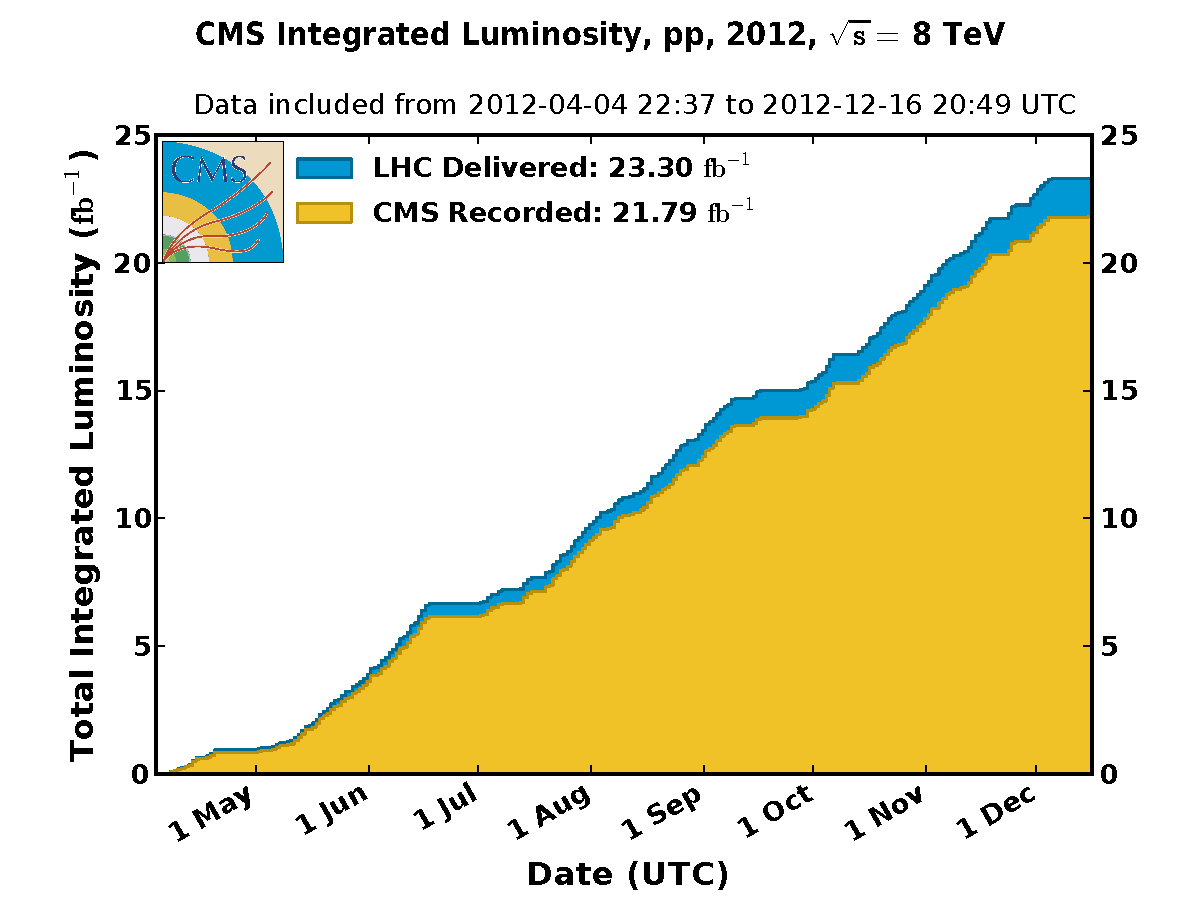
\includegraphics[scale=0.5]{THESISPLOTS/int_lumi_per_day_cumulative_pp_2012.pdf}
}
\captionof{figure}{Cumulative luminosity versus day delivered to (blue), and recorded by CMS (orange) during stable beams and for p-p collisions at 8 TeV center-of-mass energy in 2012.}
\label{fig:cmslumi}
\end{center}

%where the luminosity $\mathscr{L}$ is related to the total integrated luminosity(delivered luminosity over time) $\mathrm{L} = \int \mathscr{L}dt$ and is defined in terms of accelerator(assuming round beams and equal values of beta function) parameters as:

%\begin{equation}\label{eq:lumi}
%\mathscr{L} = \frac{1}{4\pi}\cdot\left(f_{rev}\mathit{n}_{b}\mathit{N}_{b}\right)\cdot\frac{\mathit{N}_{b}}{\varepsilon_{N}}\cdot \frac{\gamma}{\beta^{\ast}}\cdot \mathscr{R}(\theta_{c},\varepsilon,\beta^{\ast},\sigma_{z} )
%\end{equation}

%where $\mathit{N}_{b}$ is the number of particles per bunch, $\mathit{n}_{b}$ is the number of bunches, $f_{rev}$ is the revolutionary frequency, $\gamma = E/m_{p}$ is the relativistic factor, $\varepsilon_{N}$ is the normalised beam emittance which along with $\beta^{\ast}$, the value of the amplitude or beta function at interaction point, determines the size of the beam. $\mathscr{R}$ is the geometrical reduction factor arising from the fact that the beams to not collide head-on but at a non-zero angle called the crossing angle or \textit{"Piwinski angle"}( $\phi \equiv \frac{\theta_{c}\sigma_{z}}{2\sigma_{x}}$). This effect is known as the \textit{hour-glass effect}.
%From the above definition \ref{eq:lumi}, it is evident that keeping the emittance (meaning particles in beam are confined to a small distance and have nearly the same momentum ) means the likelihood of particle interaction will be greater and thus higher luminosity. However this is often not easy to archive as increasing the beam energy means reducing the beam emittance. The normalized emittance $\varepsilon_{N}$ is often used as its dependence on beam energy is a squared root dependence.
%In the same way, lower beta values implies the width of beam is narrower or properly \textit{"squeezed"} at interaction point resulting to an increase in number of collisions hence higher luminosity.
%This squeezing of depends on the quadruple magnet configuration and powering. 
%In addition to low beam emittance and lowest value of beta function at interaction point($\beta^{\ast}$), one can also archive higher luminosity by using high population bunches($\mathit{N}_{b}$) and collide them at high frequency.
%\%paragraph*{Luminosity Measurement}
%\par
%Obviously using equation \ref{eq:lumi} to determine the instantaneous and integrated luminosity would involve a lot of uncertainty in the measurements of about 20-30\%, as there are so many parameters whose value need to be measured precisely in a normal LHC operation. Rather specialised LHC runs known as \textit{"Van der Meer Scans"}\cite{lhclumi} are used to calibrate specialized equipments used for determining luminosity.
%The method employed by CMS(using TOTEM) is to use the total proton-proton~(\textit{p-p} cross section. 
%The method employed by CMS is using the Hadronic Foward~(HF) calorimeter to make luminosity measurements.
%Using production rates or cross sections of well and precisely calculable processes and rewriting \ref{eq:lumi} as:
%\begin{equation}\label{eq:LInt}
% \mathscr{L} \equiv \frac{Rate_{tot}}{\sigma_{tot}}    = \frac{\mu \mathit{n}_{b} f_{rev}}{\sigma_{tot}} 
%\end{equation}
%where $\mu = \left\langle \mathit{N}_{tot}/ \mathit{n}_{b} \right\rangle $ is the \textit{average number of interactions per bunch crossing}.

  
%of well understood and calculable processes such as the production of $\mathrm{W}$ and $\mathrm{Z}$ bosons or di-leptons via  two photon exchange. 
%\subsection{Superconducting Electromagnets}
%The LHC design and operation uses a total of 9593 powerful magnets of different types for different purposes. Since there are two beams of protons running in clock-wise and anti-clock wise directions, the LHC uses an ingenious technique design  of the magnetic field in every dipole magnet generates a vector field $\mathbb{B}$ in each pipe pointing in opposite direction to that of the other but both always perpendicular to the beam directions. The Lorentz or magnetic force acting on the protons in both pipes always point towards the center thus keeping the beams in circular motion. In circular accelerators as the LHC and its smaller synchrotron rings, given the accelerator radius,$R$, the beam energy $p$ is determined by the strength $\mathbf{B}$ of the magnetic field. This can be easily understood using the Lorentz force  such that $\displaystyle{p[TeV] = 0.3\mathbf{B}[T]\cdot R[km] }$.
%The LHC is is a 26.659~km in circumference machine using powerful dipole magnets with magnetic field strength of about 8.33~Tesla(T) are 7~TeV to keep the protons circulating in their curved path or orbits. The LHC operates using superfluid helium for heat transport at 1.4~K(-271.3~$^{\circ}C$)  temperature to prevent these near 1232 dipole magnets, 858 quadruple and 6208 correcting magnets from overheating due to the energy stored in these magnets. Conventional magnetics aren't convenient for modern particle accelerators with high center of mass energy for both performance and economic reason. Rather, superconducting magnets made with modern technology using  niobium-tantanium~(Nb-Ti) filaments strands or cables are used to provide the high magnetic field required. 
%These magnetics provide a magnetic field strength of about 8.33~T and are kept at about 1.4K in temperature during LHC operation.

%Quadrupole electromagnet and correcting magnets are  used to keep the particles in the beam and archive the required focus and de-focusing needed. At interaction point, the quadrupole magnets are held symmetrically around the beam pipe to help squeeze the proton beams to very low values of beta function thus ensuring that many particle collisions as possible necessary for higher luminosity.


%\subsection{Timing}
%The Large Hadron Collider (LHC) is designed to collide proton-proton (pp) bunches every  24.95~ns at designed luminosity. This means, the distance between each proton bunch is about 7.5~m compared to the nearly 100~m of optical fibre length which is required to transport readout information from the very front end electronics on the detectors to the back end  electronics at Point 5 for processing.
%It is therefore imperative to have a data synchronisation system for the trigger and readout systems of the LHC experiments in order that events from every proton-proton collision are properly assigned to the particular bunch crossing ~(BX) which produced them.
%The LHC is equipped with a Timing, Trigger and Control~(TTC) system with a bunch clock frequency of 40.07897~MHz whose function is to distribute synchronized LHC time to all the detectors including CMS.
%Timing synchronisation in the LHC is achieved using a Beam Synchronous Timing ~(BST) system which distributes timing using the LHC revolution frequency(at 11.246~kHz) or LHC orbit  and the RF bunch crossing frequency(40.07897~MHz at 7~\TeV). 
%Thus, the LHC fast timing signals from the RF generators  of the machine and orbit signals are distributed from the Prevessin Control Room~(PCR) through single-mode optical fibers(about 10.1~km in length for CMS) to all LHC experiments,  test beam areas, beam instrumentation around the ring and the SPS transfer lines.  At CMS counting room, the LHC clock and orbit signals  are recovered in the TTC Machine Interface crate~(TTCmi) and later distributed to the Trigger Control and sub-detector master TTC crates. All Level1~(L1) trigger and Data Acquisition~(DAQ) pipelines are driven with a 24.95~ns cycle clock locked to the LHC machine clock. The phase difference between the LHC 40~MHz clock and the arrival of detector signals from collision to the front-end electronics must be determined and adjusted for and monitored. The determination and assignment of pulses to bunch crossings depends critically on this initial clock phase adjustments and stability. This amplitude or pattern(also known as trigger primitives) for each trigger and bunch crossing is transmitted to the regional trigger logic in digital form every crossing and is synchronised with the LHC clock. Each trigger primitive digital data is then assigned to clock cycle in a process known as bunch crossing assignment. a   Detail expert description of LHC unified timing distribution system can be found here \cite{LHCT, LHCT1, LHCT2, LHCT3}.
%This means that there is the possibility of producing a LL particle when two protons collide every 25~ns.
%Thus it becomes a serious challenge  for triggering, data acquisition and associating the correct emerging particle to
%the correct bunch crossing (BX).
 %This is even more challenging for LL particles produced with low velocity since
%by design and read-out, with the time separation of 25~ns between BXs,
%Particles produced from LHC are assumed to be travelling at the speed of light (c = 299 792 458~m$s^{-1}$).
%Thus, such light speed particles will travel a distance of $\approx 7.5$~m.
%This leads to the possibility of having about 3 BXs  simultaneously contained in the Compact Muon Solenoid~(CMS) detector.
%As a result, LL particles produced with slower velocity might cause triggers to assigned particles to the wrong BX and so reduced the trigger
%efficiency for LL particles. An interesting study has been done by the another multi-purpose detector at CERN, ATLAS
%which looked at LL particle with different velocities~ $\beta$ and showed that it is important to enlarge triggering windows so as to increase
%triggering efficiencies for low velocity particles.

\subsection{LHC Bunch Structure}
%An LHC orbit is made of about 3564 \textit{bunch} places. However only 2808 are occupied with protons. The bunch structure is archived by  breaking a continuous proton beam into pulsed beam of separate bunches using an electromagnetic field  with oscillating frequency of 400~MHz(LHC ring) in the SPS and LHC RF cavity. Thus each bunch is in an RF bucket. 
Each LHC proton bunch is placed inside an RF buckets during beam filling. % with where each RF bucket has an energy against time profile as can be seen in figure below.
The filling scheme is such that not all RF buckets have proton bunches. 
Those empty buckets or beam gaps are necessary to avoid parasitic collision near IP and to make room for beam dump and beam halos known as beam cleaning.%the rise/fall times at the SPS/LHC injection and ejection and to abort kickers magnets during
The separation in time between two buckets/bunches filled or unfilled is approximately $2.5$~ns. There are  about $10^{11}$ protons per bunch during filling and acceleration.
 %Filling and acceleration at each RF cavity point is performed so that there are 
However, during filling and eventual bunch splitting at PS, it is possible that some empty buckets are filled with a much smaller proton population compared to the main bunch. These buckets with few protons can be either trailing the main bunch by $\Delta t$ = 2.5, 5.0, 7.5, $\ldots$~ns, or leading the main bunch by $\Delta t$ = -2.5, -5.0, -7.5, $\ldots$~ns. If these less populated bunches are $2.5$ to $3.0$~ns spaced in time from each other, they are referred to as \textit{satellite} bunches and if $5.0$~ns, they are referred to as \textit{ghost} bunches. Figure \ref{fig:LDM-Ghost} shows ghost and satellite bunches and a main proton bunch.
\begin{center}
\centering
\mbox{
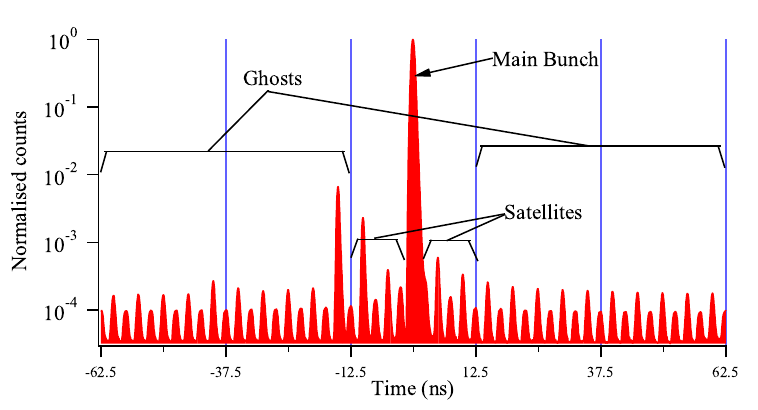
\includegraphics[height=0.5\textwidth, width=0.85\textwidth]{THESISPLOTS/Ghost-Satellite-Bunches-LDM.png}} 
\captionof{figure}{Longitudinal Profile taken with Longitudinal Density Monitor~(LDM) detector showing definition of Ghost/Satellite bunches with respect to main bunches.}
\label{fig:LDM-Ghost}
\end{center}
The presence of ghost/satellite bunches increases the uncertainty in LHC luminosity measurements and can also generate proton-proton interactions near but not at the collision region. Effects on ghost/satellite bunches on instantaneous luminosity measurements have been studied 
using CMS, ATLAS and ALICE detectors.  Their results showing clear observation of physics events produced from
ghost and satellite bunch collisions is shown in figure \ref{fig:CMS-ATLAS-Ghost}.
CMS uses energy deposits in the endcap calorimeters to observe time space which is consistent with the expectation from ghost/satellite bunches while in ATLAS
 uses the Longitudinal Density Monitor~(LDM)detector to study ghost/satellite bunches. 
\begin{center}
\centering
\mbox{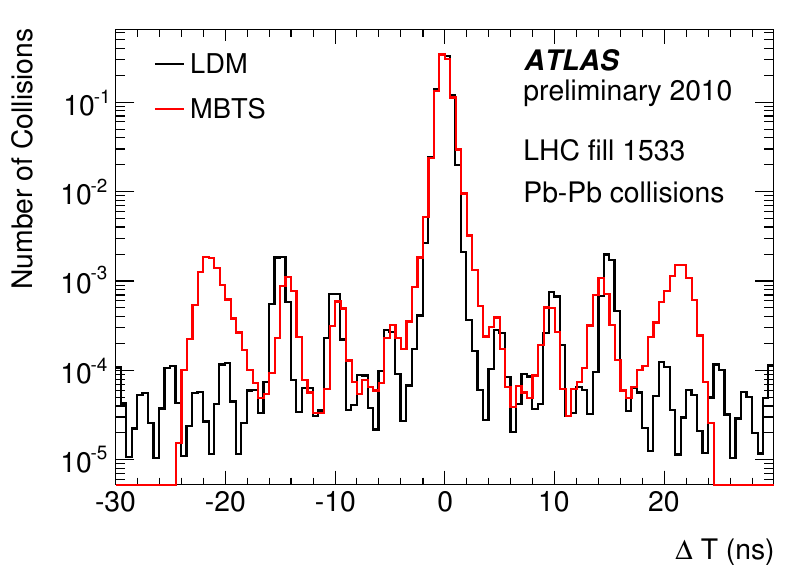
\includegraphics[height=3.0in,width=2.5in]{THESISPLOTS/ATLAS-LDM-GHOST.png} \quad \quad
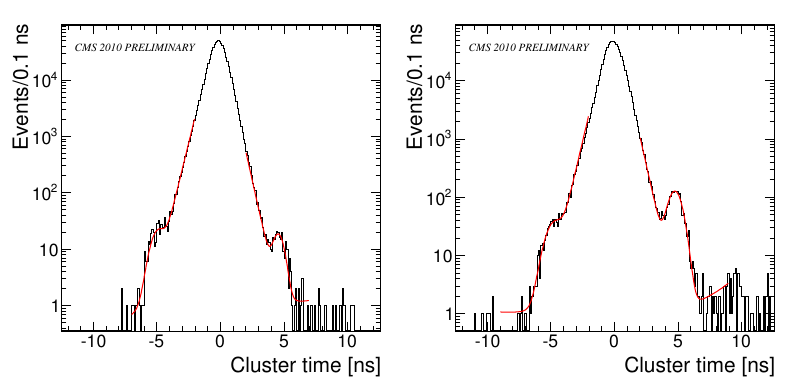
\includegraphics[height=3.0in,width=3.0in]{THESISPLOTS/CMS-Ghost-Profile.png}} 
\captionof{figure}{(left)Arrival time distribution(red) of ATLAS MBTS  for LHC fill 1533 during 2010 Pb-Pb run and LDM profile(black) for Beam2(same for Beam1).\newline
(Right) Timing of Clusters in the CMS endcap calorimeters for fill 1089:Left: EEP detector(left side of IP $z> 0$) Right: EEM detector( right side of IP, $z<0$).  Plots from ATLAS \cite{ATLAS-GHOST} and CMS, \cite{CMS-GHOST}}
\label{fig:CMS-ATLAS-Ghost}
\end{center}
%There is the possibility that ghost/satellite - ghost/satellite and ghost - Beam1/Beam2 collisions will happen generating events at the CMS detector. This is a major background in the search for delayed photons or objects in general as these collisions can occur \textit{in-time}(Beam1- Beam2) collisions or \textit{out-of-time} collisions. It is thus imperative to be able to quantify this contributions in any search analysis. We will show in future studies we have performs to both \textit{"guestimate"} and quantify these contributions in our search analysis.
Table \ref{tab:tableLHC} gives a summary of the LHC design conditions compared to the conditions used during the LHC RUN 1 operation. 
\begin{center}
%\begin{sidewaystable}
 \begin{table}[H]
  \begin{turn}{90}
  \centering
 %\setlength{\abovecaptionskip}{0pt}
  %\setlength{\belowcaptionskip}{10pt}
 % \topcaption{GMSB,GGM Phenomenology and Relevant final states}
 %\rotatebox{90}{%
  \begin{tabular}{l|l|l|l|l}
  %\hline \hline
  \multicolumn{5}{c}{\bfseries{LHC Operation Parameters 2010-2013}} \\
  \hline
  \toprule
  \bfseries{Parameter} & \bfseries{2010 value} & \bfseries{2011 Value} & \bfseries{2012/13 Value} & \bfseries{Design Value} \\
   \hline \hline
   Beam energy[Te] & 3.5  & 3.5  & 4.0  & 7 \\ 
  \hline
  $\beta^{\ast}$ in IP 5[m] & 3.5 & 1.0 & 0.6  & 0.55 \\
  \hline
   Bunch spacing [ns]& 150 & 75/50 & 50 & 25 \\
  \hline
  Number of bunches & 368 & 1380 & 1380 & 2808 \\
  \hline
  Protons/bunch  & $1.2 \times 10^{11}$ & $1.45 \times 10^{11}$ &  $1.7 \times 10^{11}$& $1.15 \times 10^{11}$ \\
  \hline
  Normalised emittance[mm.rad] & $\approx 2.0$ & $\approx 2.4$ & $\approx 2.5$ &  3.75\\
  \hline
  Peak luminosity[$cm^{-2}s^{-1}$]& $2.1 \times 10^{32}$ & $3.7 \times 10^{33}$ & $3.7 \times 10^{33}$ & $1 \times 10^{34}$ \\
  \hline
  Evts/bunch crossing & 4 & 17 & 37 &  19 \\
  \hline
  Stored Beam energy(MJ)& $\approx 28$ &  $\approx 110$  & $\approx 140$  & $\approx 362$ \\
  \hline
  Int. Luminosity by CMS[$pb^{-1}$]&  &  &  &  \_ \\
 \hline
 Circumference[km]  &26.659 & 26.659 & 26.659 & 26.659 \\
 \hline
 Dipole Magnet B[T] & 8.33 & 8.33 & 8.33 & 8.33 \\
 \hline  
  \bottomrule
  \end{tabular}
   \caption{LHC operation parameter conditions during RUN 1, 2010-2013}
   \label{tab:tableLHC}
 %\end{sidewaystable}
   \end{turn}
  \end{table}
\end{center}


\clearpage

\section{Compact Muon Solenoid}
\subsection{Overview}
The Compact Muon Detector~(CMS) is a modern particle detector design for many different particle detection capability.
It is one of the general purpose detectors located at one of the proton-proton collision points along the 27~\km LHC ring.
It's main feature is the presence of a superconducting solenoid of 6~\m internal diameter providing a field of 3.8~T for measuring a charge particle's momentum as the particle bends under the influence of this field traveling in the detector.
%The goal of the  Compact Muon Solenoid~(CMS) detector is to identify particles by measuring their energies, momenta and track if applicable, as they pass through the detector. It is for this reason that the CMS apparatus is a general purpose particle detector operating about 330 feet underground at  point 5~(P5)LHC in cessy,France. . 
This magnetic field  encloses an entirely silicon pixel and strip tracker detector use for vertex finding and for detecting and reconstructing the tracks of charged particles, a lead-tungstate scintillating-crystals electromagnetic calorimeter (ECAL) and a brass-scintillating sampling hadron calorimeter (HCAL). Very long lived particles like muons are measured in gas-ionization detectors embedded in the flux-return iron-yoke located at the outermost section of the detector.
It has a simple cylindrical structure consisting of barrel and endcap detectors and an extensive forward calorimetry and detectors to provide a near $4\pi$ solid angle coverage assuring good hermetic particle detection. The CMS apparatus has an overall length of 21.6~m, a diameter of 14.6~m, and weighs 12,500 tons. Figure \ref{fig:CMS-DET} shows the CMS detector indicating the different sub-detectors and their 
material design type. We provide a performance summary and  material type of each sub-detector in Table \ref{tab:tableCMS} of the CMS detector.
The CMS uses a coordinate system with the origin coinciding with the center of the detector where proton-proton or nominal collision 
occurs. This point is commonly referred to as the \textit{interaction point}~(IP). The direction of $x,y,$ and $z$-axes are as shown in figure \ref{fig:CMSDCORD}. However, for particle identification, CMS uses a more convenient coordinate system based on the polar coordinates. In this polar coordinate system, the azimuthal angle, $\phi$, is measured in the $x-y$ plane, where $\phi = 0$, is the $x$-axis and $\phi = \pi/2 $, the $y$-axis. The radial distance in this plane is denoted $R$ and the polar angle $\theta$  measured from the $z$-axis is related to \textit{pseudo-rapidity}, $\eta$, through the relation; $\eta = -\ln \tan(\frac{\theta} {2}) $. 
The coordinate system $(\eta, \phi)$ and its radial distance $R$ identifies a point in the cylindrical volume of the CMS detector. 
In the coming sections, we describe the geometry, material characteristics and functionality of the CMS subdetectors  used in our analysis.

\clearpage
\begin{center}
\centering
\mbox{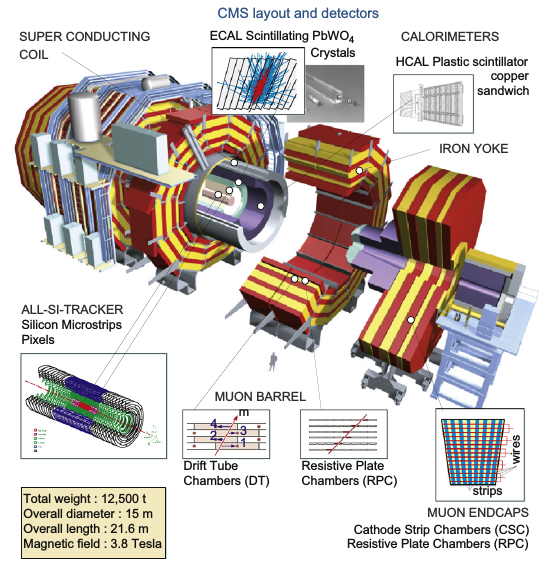
\includegraphics[width=10cm]{THESISPLOTS/CMS_LAYOUT_AND_DETECTORS.png}} 
\captionof{figure}{CMS Detector showing the different subdetectors and their material.}
\label{fig:CMS-DET}
\end{center}

\begin{center}
\centering
\mbox{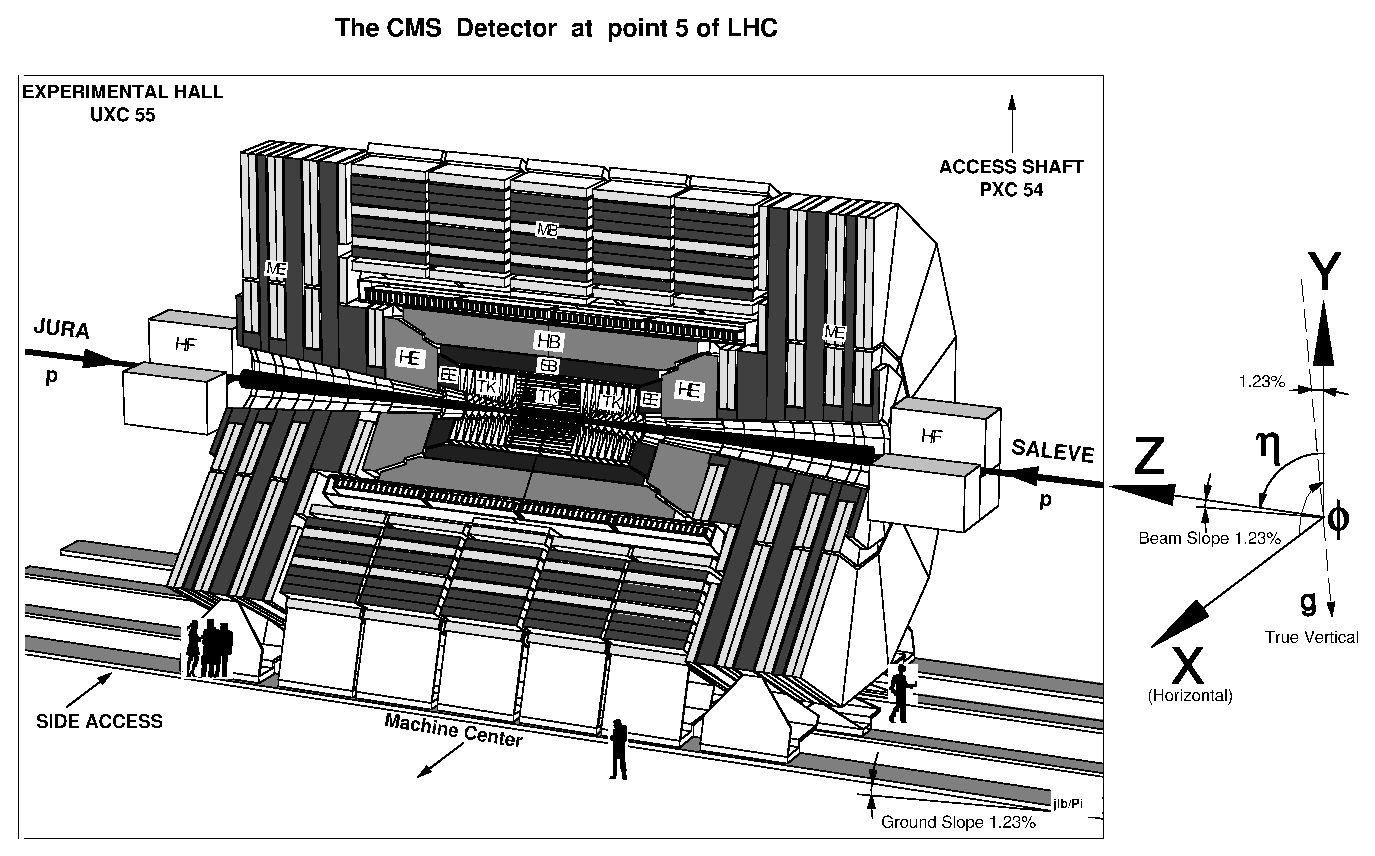
\includegraphics[scale=0.5]{THESISPLOTS/CMS_DETECTOR.eps}} 
\captionof{figure}{CMS detector schematic view with definition of $x-y-z$ coordinates.}
\label{fig:CMSDCORD}
\end{center}

\begin{center}
\centering
 %\setlength{\abovecaptionskip}{0pt}
  %\setlength{\belowcaptionskip}{10pt}
 % \topcaption{GMSB,GGM Phenomenology and Relevant final states}
  \begin{tabular}{l|l|p{3.2cm}|p{3.9cm}}
 % \hline \hline
  \multicolumn{4}{c}{\bfseries{CMS Detector and Resolution}} \\
  \toprule
  \bfseries{Subdetector} & \bfseries{Quantity} & \bfseries{Resolution} & \bfseries{Uses}  \\
   \hline \hline
 Tracker   & Momentum[GeV/c]  & $\sigma_{T}/p_{T} \approx 1.5\times 10^{-4}p_{T} + 0.005$ & \mbox{Silicon Pixels and Strips} \\ 
  \hline
  ECAL   & Energy[GeV] & $\sigma/E \approx 3\% /E + 0.003$ & $\pb$ Crystals \\
   ECAL  & Time[ns] & $\sigma(\Delta t)= \frac{N}{A_{eff}/\sigma_{n}}\oplus\sqrt{2}\bar{C} $ & $\pb$ Crystals \\
  \hline
  HCAL & Energy[GeV] & $\sigma/E \approx 100\% /E + 0.05$ & Brass + Scintilator\\
  \hline
  Muon Chambers & Momentum[GeV/c] & $\sigma_{T}/p_{T} \approx$ 1\%  \@ 50 GeV to  10\% \@ 1 \TeV & inner tracker + Muon Systems \\
  \hline
  Magnetic field & B-field strength[T] & 3.8~T + 2~T & Solenoid + Return Yoke\\
  \hline
  Triggers  & On/Off-line & Levels &\mbox{L1(On-line)} +\mbox{HLT(Off-line)}(L2+L3) \\
  \hline
   \bottomrule
  \end{tabular}
  \captionof{table}{CMS detector material, \cite{CMSTDR}, and resolution(Time resolution: $N\approx 35$~ns, $\bar{C}\approx 0.070$~ns  \cite{ECALTIME2014}) }
 \label{tab:tableCMS}
 \end{center}
%\subsection{Tracker}
%Particles produced from proton-proton collision traverse the tracker sub-detector first. The job of the tracker is to measure the trajectory of charged particles, which are curved because of the magnetic filed produced by the magnetic coils. By measuring the curvature of these particle, the particle's momentum can be measured and its charge determined. The tracker is a silicon based detector and thus operates under the concept of ionization. It occupies a volume of 2.4~m in diameter and 5.4~m in length, consisting of pixel and strip sections geometrically arrange in cylindrical layers of barrel and disc-shaped endcaps, enclosed within the calorimeters. These sub-detectors all sit inside the 6~m in diameter solenoid magnet operating at 3.8~T. Figure \eqref{fig:CMSTRAK} depicts a schematic picture of the tracker with three barrel layers covering a region of radius from 4~cm to 15~cm in radius and two endcap discs within 49~cm on either side of the collision point along the $z$ axis; ten barrels layers  and twelve endcap disks per side of silicon strip detectors covering a region with radius from 15 to 110~cm and within 280~cm on either side of the LHC beam axis. The total tracker acceptance region in pseudo-rapidity is $|\eta| < 2.5$. The pixel detector is used for identifying the primary and secondary vertices of particles while the inner tracker of strip detector is for tracker reconstruction. 
%\begin{center}\label{CMSTRAK}
%\centering
%\mbox{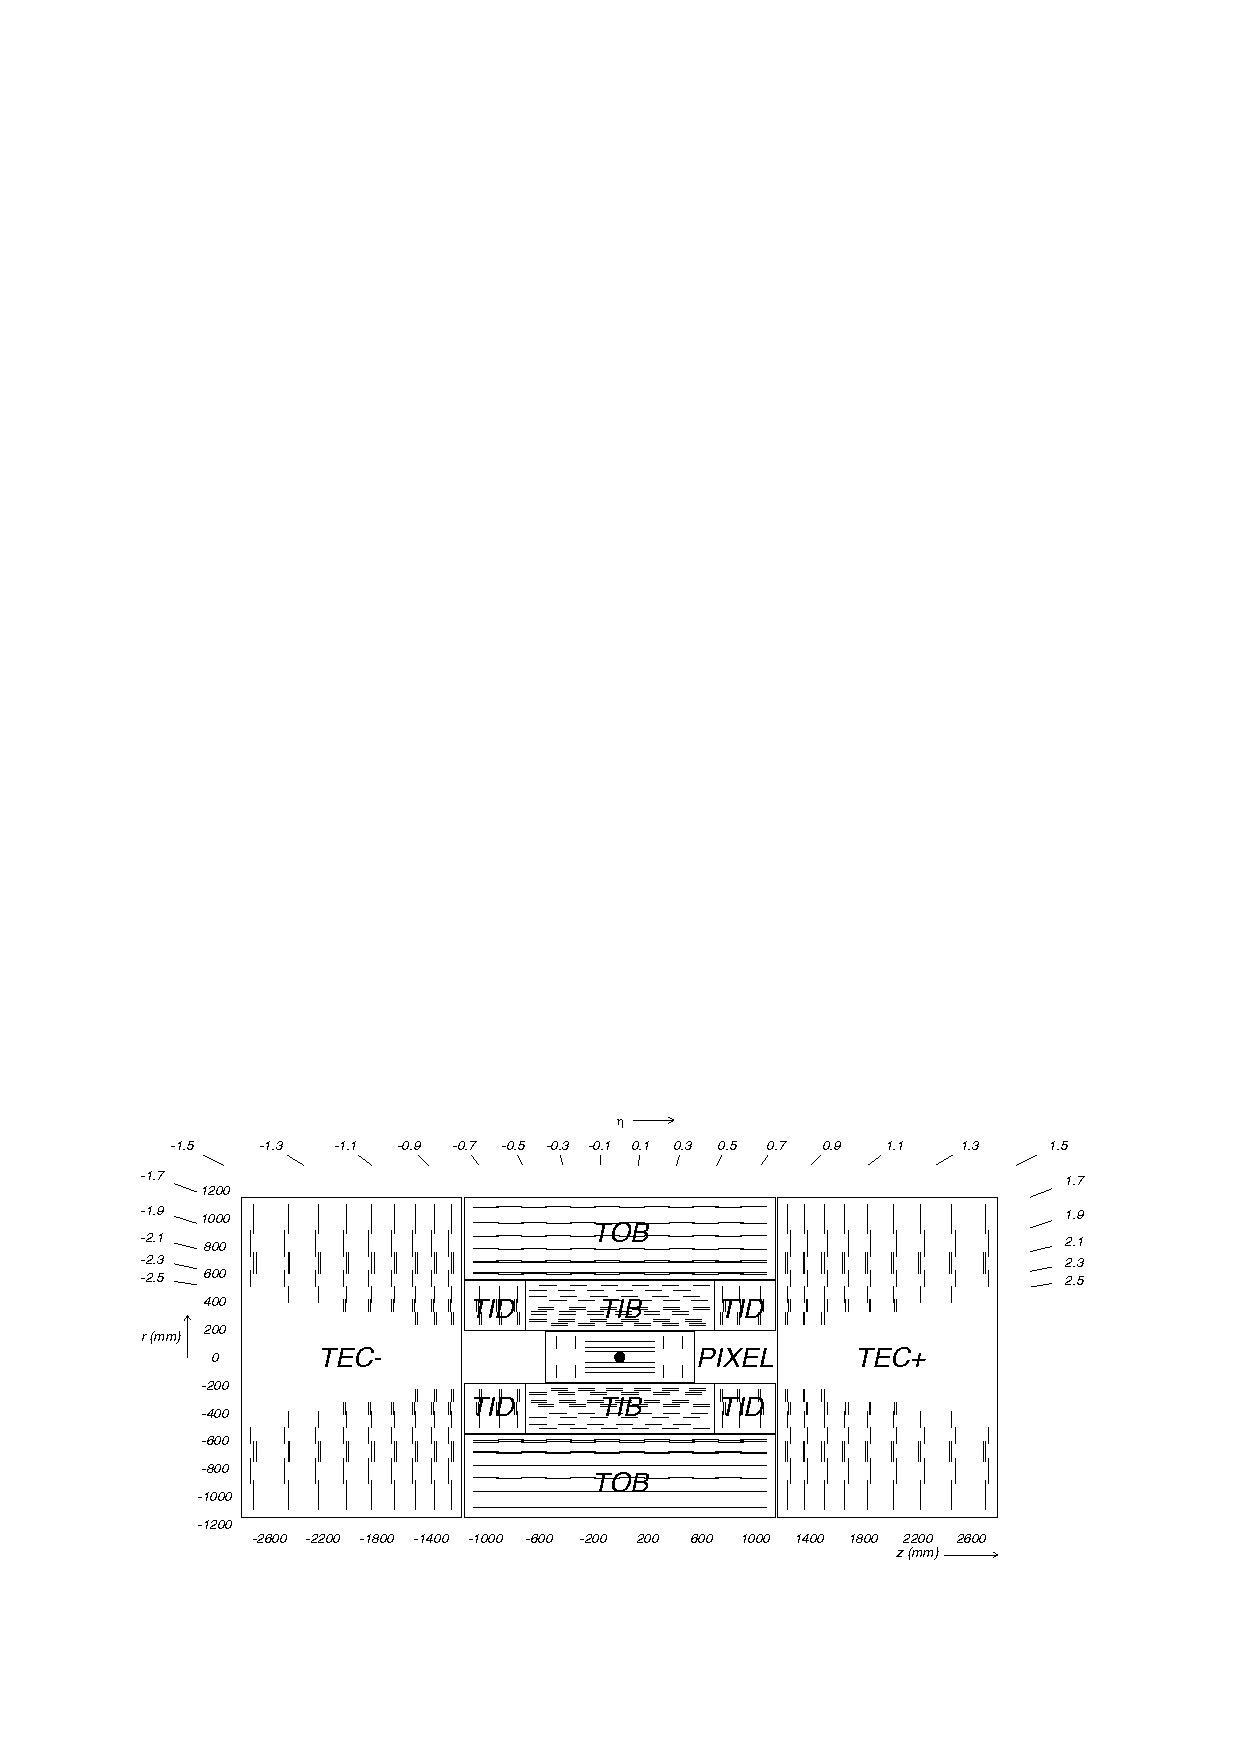
\includegraphics[scale=0.6]{THESISPLOTS/Tracker.pdf}} 
%\captionof{figure}{Schematic diagram of CMS Tracker showing the silicon pixel detector region~(inner closer to LHC beam) and silicon strip reigion~(outer).}
%\label{fig:CMSTRAK}
%\end{center}
%\subsubsection{Pixel}
%The pixel vertex detector occupies the inner most region, very closed to the interaction region. Providing high-resolution and three-dimensional patterns of space points using silicon pads as pixels, the primary vertex and secondary vertices arising from the decay of heavy and relatively long-lived particles such as B-mesons containing b-quarks can be identified. This is also known as impact parameter measurements. The pixel covering a region of pseudo-rapidity $|\eta| < 2.4$ compliments the track finding by providing additional space points to seeding hits in the inner tracker.  Each pixel has a size of $100\times150$~$\mu m^2$ 
%covering a total area of $\approx 1~m^{2}$ and there are 66 million pixels read out by 16000 readout chips on the silicon sensors. The pixel is organised in three 53~cm long barrel layers~(Pixel Barrel=PXB), positioned at radii  of 4.4, 7.3 and 10.2~cm and two disks each per side (Pixel Forward=PXF), placed at $\pm 34.5$~cm and $\pm46.5$~cm from the interaction point and covering a radii between 6 and 15~cm. This guarantees each charged particle track crosses at least two layers of pixels.
%This arrangement ensures that the pixel detector provides  precise tracking points in the $ r-\phi$ and $z$ responsible for small impact parameter resolution of about $\sim 15~\mu m$. Small impact parameter resolution is important for precise secondary vertex  reconstruction and position resolution crucial in the identification of objects produced with displaced vertices with life-time of  about $\tau \approx 10^{-12}~s$ like mesons such as $B^{0,{\pm}}$, $D^{0,{\pm}}$, $\tau^{\pm}$, which may travel a distinguishable distance (c$\tau$ $\approx 100~\mu$m before decaying. Because of very high radiation dose of about 100~Mrad absorbed by the pixel detector, there is currently upgrade of the complete pixel detector in preparation of LHC Run 2.

%\subsubsection{Silicon Strip Tracker}
%CMS silicon inner tracker surrounding the pixel detector allows for the tracks of promptly produced charged particles with $\PT = 100GeV/c$ to be reconstructed with a resolution in the transverse momentum \PT  of about $\sim 1.5\,\%$. High momentum particles are less curved by the magnetic field than low momentum particles. Therefore, the tracker works complimentary with the calorimeter and muon detectors to ensure improve momentum resolution at all particle energies.
%The silicon micro strip tracker covers a tracking volume up to radius of 1.2~m with a length of 5.6~m. It is organised in three parts: The inner tracker with four barrel layers (Tracker Inner Barrel=TIB) and three disks per endcap~(Tracker Inner Disks=TID), 6 outer barrel layers~(Tracker Outer Barrel=TOB) closed by 9 wheels on both sides.~(Tracker EndCap=TEC). 
%The silicon strip is made of 15148 silicon microstrip detector modules. Each module has a set of sensors. It occupies an active area of $200~m^{2}$ providing a coverage in pseudo-rapidity up to
% $|\eta| < 2.5 $.
% The TIB/TID delivers up to 4 $r-\phi$ measurements on a trajectory using 320~$\mu$m thick silicon micro strip sensors arranged  parallel to the beam direction in the barrel and radial on the disks. The strip pitch is 80~$\mu$m on layer 1 and 2 and 120~$\mu$m on layer 3 and 4 of the TIB, leading to a single point resolution of 23~$\mu$m and 35~$\mu$m, respectively. The TID also have varying pitches with both the TIB/TID enclosed by the TOB. The layering structure can be seen figure \eqref{CMSTRAK}. The nearly 9.6 million silicon strips provide a spatial resolution measured to be about $10~\mu$m for $r-\phi$ measurement and about $20~\mu$m for $z$ measurement necessary for particle trajectory reconstruction.
%The combined pixel and micro strip modules allows for nearly 75 million readout electronic channels in the tracker.
 

\subsection{Calorimeter}
A CMS calorimeter absorbs a good fraction of energy of an incident particle and produces a signal with an amplitude proportional to the energy absorbed. This absorption is through the cascade production of secondary particles with energy of the incident particle directly proportional to the number of secondary particles produced. The are two types of calorimeters choices used in the CMS detector; the \textit{Electromagnetic calorimeter}~(ECAL); for absorbing the energy of electromagnetic particles such as photons and electrons and a \textit{Hadronic calorimeter}~(HCAL) made of more than one type of material for stopping and absorbing the energy of hadrons such as kaons and pions through strong interactions. The combined calorimeter detectors of CMS covers a region in $|\eta| < 5 $ making it nearly hermetic for good missing energy measurements. The ECAL and HCAL are arranged in a nested fashion shown in figure \ref{fig:ECAL-HCAL} so that electromagnetic particles can be distinguished from hadronic particles by comparing the depth of the particle shower penetration in both calorimeters.

\begin{center}
\centering
\mbox{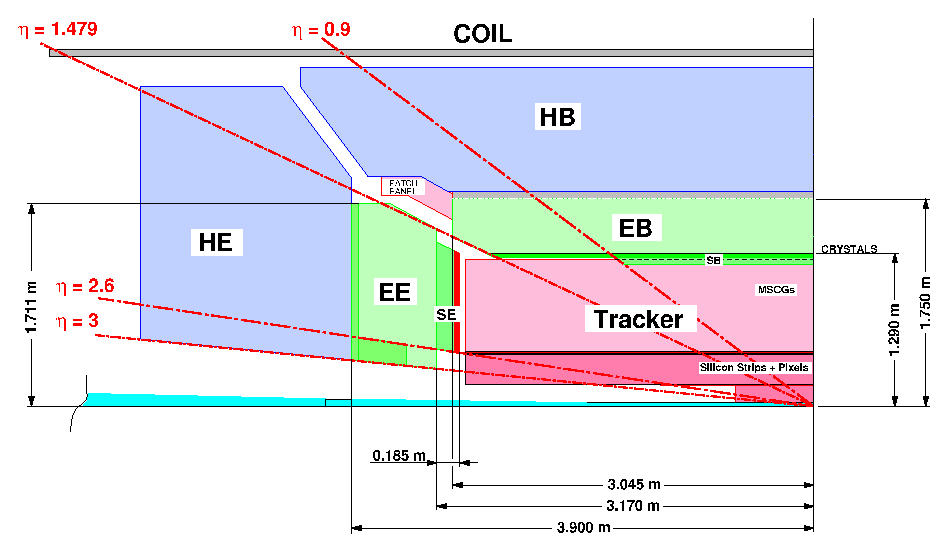
\includegraphics[scale=0.5]{THESISPLOTS/ECAL-HCAL.eps}} 
\captionof{figure}{Schematic diagram of CMS calorimetry system with HCAL enclosing ECAL in the Barrel and Endcap regions.}
\label{fig:ECAL-HCAL}
\end{center}

\subsubsection{Electromagnetic Calorimeter}
 The electromagnetic calorimeter~(ECAL) detects photons and electrons. High energy photons and electrons are detected through their interaction with the lead tungstate~(\pb) crystals. 
During this interaction which happens either through electromagnetic showering or electron-positron pair production~(\textit{bremsstrahlung}), the incoming photon or electron deposit practically almost all of its energy.
There are 75848 crystals in total mounted in a cylindrical geometry, with a barrel~(\textsc{EB}) and an endcap~(\textsc{EE}) structure.   
 % The choice of \pb is due to its high density which allows for fast scintillating time of nearly 18~ns, has a fine granularity to enhance good resolution and is radiation resistant which are important characteristics in an LHC environment.
The choice of \pb crystals as calorimetry material by CMS for operation in the LHC environment is because of its a high density~(8.28~g/$\cm^{3}$), short radiation length~($X_{0}$=0.89~\cm) and a small Moli$\grave{e}$re radius~(22~\cm). In a high radiation dose and fast timing~(25~ns proton bunch spacing) environment like the LHC, \pb crystals is preferred to other crystal materials for its high radiation resistance and a scintillation decay time which is comparable to the LHC bunch crossing interval of 25~ns and about 80\% of the light is emitted in 25~ns.  
The probability of an electromagnetic object with high energy to interact either through \emph{Bremsstrahlung} or \textit{pair production} with the material in ECAL is proportional to the nuclear charge, \text{Z}, of the material. \pb is a high \text{Z} material and this makes it once more the preferred material choice for electromagnetic calorimetry by CMS. The small Moli$\grave{e}$re radius ensures that on average about $95$\,\% of the electromagnetic shower energy is contained within a crystal crystal volume of about 9 crystals. This reduces the transverse spread of the electromagnetic cascade from multiple scattering of electrons and helps improve on  the estimation of the transverse position of impact of an incident particle. It also provides a fine granularity for measuring
the particle's energy by providing fewer overlap of particle signals. Its dense nature also allows for the electromagnetic shower to develop early and therefore likely to be fully contained within a compact device like CMS.
%thus ensuring good precision for measuring the energy of an incoming electromagnetic particle and thus better energy resolution. 
 
The EB section of the ECAL covers a pseudo-rapidity of $\vert \eta \vert< 1.479 $. It has 61,200 crystals providing a granularity of 
$360$ degree fold in $\phi$ and $(2 \times 85)$-fold in $\eta$.The crystals are mounted in a quasi-projective geometry so that their axes make an angle of 3\% with respect to a line vector from the nominal interaction vertex in $\eta$ and $\phi$ directions. This avoids cracks aligned with a particle's trajectory. A crystal in EB is approximately 0.0174~$\times$~0.0174 in $\eta-\phi$ or 22~$\times$ 22~$\mm^{2}$ at its front face and 26~$\times$~26~$mm^{2}$ at its rear face. Each crystal is 230~\mm long corresponding to about 25.8~$X_{0}$ radiation lengths. The crystal's radial distance measuring from the center of the face of the crystal to the beam line is 1.29~m. A number of crystals are placed in a thin-walled alveolar structure made with aluminum forming a \textit{submodule}.  
Each submodule is arranged into 4 modules of different types according to their $\eta$ position. There are about 400 to 500 crystals in each module and these 4 combined make one \textit{supermodule} containing 1700 crystals.
To reduce crystal reflective lost, the aluminum surface is coated to avoid oxidation leading to coloration.
On the rear end of each EB crystal, two \textit{Avalanche Photodiodes}~(APD)  is glued to collect the scintillating light from the crystals converting light into charge current which is further collected by the read-out electronics.
 \newline
The endcap sector covers a pseudo-rapidity region of $1.479 <\vert \eta \vert < 3.0$ with a Preshower~(\textsc{ES}) detector made of silicon strip sensors interleaved with lead placed immediately in front of it. The purpose of the preshower is to identify photons from the decay of neutral pion, $\Ppizero \rightarrow \Pphoton\Pphoton$ and also to help separate photons producing electrons through pair production from photons not producing electrons before their arrival at the EE. 
The endcap located on the $+z$ side of the nominal interaction is denoted \textsc{EE}$+$ while the other located on the $-z$ side  is denoted as \textsc{EE}$-$. The longitudinal distance between the IP and the center of the surface of the \textsc{EE} crystals is $3.154$~\cm. Each endcap is divided into two halves called \textit{Dees} with each Dee holding 3662 crystals. 
Crystals in \textsc{EE} with identical shape are grouped into 5~$\times$~5 units called \textit{supercrystals}~(SC). 
The crystals in the SC form an $x-y$ grid. Each crystal is 220~mm~(24.7~$X_{o}$) in length and has a front face and rear cross section of 28.62~$\times$~28.62~square~\mm and 30~$\times$~30~square~\mm, respectively. 
Vacuum Phototriodes~(VPT) instead of APDs is glued on the rear face of each crystal for scintillating light  conversion into electrical signals. The VPT is used in the \textsc{EE} because of its high resistance to radiation and smooth operation in a strong magnetic field environment. These APDs and VPTs are used because of their high gain relative to regular photodiodess with no gain and the fact that they are not affected by the high magnetic field. Although the light yield for \pb crystals is rather low~($\approx 70$photons/\MeV), these photo-detectors have internal gain~($50$ for APDs and 10 for VPTs) and quantum efficiency of $75$\,\% for APDs and $20$\,\% for VPTs of the emission wavelength. This makes it possible that signals from incident particles with energies of a few to high \GeV longer than noise.
 
The signals from the APDs and VPTs are digitized by voltage-sensitive analogue-to-digital converters and through fibre-optic links transported as light signals to the counting room located adjacent to the experimental cavern.
\newline
The energy resolution and geometry structure of the ECAL ensures that the photon or electron's arrival energy, time, position and even the direction through the shape of its electromagnetic shower in the crystals can be identified and measured with good precision.
%Photodiodes like APDs and VPTs are similar to silicon photodiodes, with the exception that they have a buried p-n junction reversed-biased at a very high electric field. The photo electrons arriving at the junction undergo avalanche multiplication giving the device a gain.

%This homogenous design of the ECAL provides it with a performance which is optimal(by design) in its potential to discover a Higgs in the mass region 
% less than $130$\GeV/$c^{2}$ through the decay $\displaystyle{H\rightarrow\gamma\gamma}$. 
% Homogenous design implies reduced noise in the detector  thus better resolution since only a single material type is in use.
%ECAL has a current  timing resolution better than 500~ps for large energy deposits(more than 10-20~GeV in the \text{EB})~\cite{TIME} 
%and an energy resolution of ${\displaystyle\sigma/E\approx 0.45\,\%}$ for unconverted photons with energies above 100~GeV~\cite{CMSTDR}.
\subsubsection{Hadronic Calorimeter}
%Hadrons like protons, neutrons kaons and pions are unlike electromagnetic particle strongly interacting~(strong force is the force that binds nuclei together). A hadronic shower is formed when an incident hadron undergoes an inelastic collision with the nucleus of the absorber material producing secondary hadrons which as they go through successive layers of absorber material interact inelastically with other nuclei to produce further hadrons etc. 
%The  hadronic cascade loses about 30\,\% of incident hadron energy through nuclear excitation of the nuclei of atoms of the  absorber material.  Hadronic showers start to develop later with more lateral spread and and larger in the longitudinal dimensions than electromagnetic showers. 

The CMS Hadron Calorimeter~(HCAL) is comprised of four distinct subdetectors: the Barrel~(\text{HB}), the Endcap~(\text{HE}), the Outer Barrel~(\text{HO}), and the Forward~(\text{HF}). Unlike the ECAL, the HB,HE and HO subdetectors are scintillator-sampling calorimeters with embedded wavelength shifting fibers~(WLS). 
HB, HE and HO uses brass plates as the inactive material and plastic scintillator with WLS as the active material. 
The brass plate is used for absorbing the hadronic shower which comprise of an \textit{electromagnetic}(particles like $\Ppizero$s, $\Peta$s and other mesons generated in the absorption process and decay to $\Pphoton$s which develop electromagnetic~(em) showers) and \textit{non-electromagnetic} components.  The plastic scintilator is divided into $16$ $\eta$ sectors resulting in segmentation of
 $\Delta\eta\times\Delta\phi=0.087 \times\ 0.087$. It was chosen for its long-term stability and moderate radiation hardness.
energy. The scintillating light through the WLS brings the light to hybrid photodiodes~(HPDs) in the HB and HE. HPDs which have high
electrical noise and will be replaced with silicon photon multipliers~(SiPM) which have low noise during the current CMS detector upgrade. 
The \text{HB} and \text{HE} combine cover a region in pseudo-rapidity of $\vert \eta \vert < 3$. 
The HB covering the region $|\eta| < 1.3$, is divided into two-half barrel~(HB+ and HB-) sections each composed of 18 identical $20^{o}$ wedges in $\phi$. Each wedge is made of flat brass alloy and steel(only front and back plates) absorber plate.
HE covers $1.3 < \eta < 3.1$ and has plastic scintillation tiles with granularity of  $\Delta\eta\times\Delta\phi=0.087 \times\ 0.087$ for $|\eta| < 1.6$ and  $\Delta\eta\times\Delta\phi=0.17 \times\ 0.17$ for $|\eta| > 1.6$.
The HO is an extension of HB outside the solenoid and thus utilizes the solenoid coil as an additional absorber. It is used to
identify the starting shower and to measure the shower energy deposited after HB.
% to absorb the hadronic shower and sits parallel to beam axis with the innermost and outermost layers made up of stainless steal interleaved by plastic scintillating tiles.
The first active layer of the scintillating tiles is situated directly behind the ECAL in order to actively sample low energy showering particles from the support material between the ECAL and HCAL. 
%Each scintillating tile has a size of $\Delta\eta\times\Delta\phi=0.087 \times\ 0.087$ and is instrumented with a single wave length shifting fiber(WLS) for collecting the light. The summed light optical signals is converted into fast electronic signals by photo-sensors called  hybrid photo-diode(HPD).
%This in-homogeneous design gives the HCAL, an energy resolution of ${\displaystyle \Delta E/E \approx 0.5/\sqrt{E(GeV)} }$ for particles with energy above 250~GeV, much lower compared to that of homogeneous ECAL detector.
\newline
The \text{HF} occupies a pseudo-rapidity region of $3 < \vert \eta \vert < 5$.
Its purpose is to provide a closer to $4\pi$ hermetic phase space coverage required for missing transverse energy calculation or \text{MET}. MET is the established signal for very weakly interacting particles like neutrino and supersymetric particles like gravitino which travel through the detector undetected. %HF calorimeters placed upstream also have scintillating tiles called \textit{Beam Scintillation Counters}~(BSC) which in coincidence with the \textit{beam pick-up monitors}~(BPTX) detector help eliminate beam background contamination at the trigger level. 
HF consists of radiation hard quartz fibers embedded in steel absorbers running parallel to the beam axis. The signal from Cherenkov light emitted in the quartz fibers in response to charged particles makes it possible to detect all charge particles in the forward region. The HF calorimeter has long and short fibers for better sampling and to distinguish showers generated by electrons and photons from those generated by hadrons.
%The goal of this hardware design is to give better compensation for different shower components in the hadronic shower.
 The choice of quartz fibers is because of its high resistance to the high radiation in the forward detectors and its fast production of light through Chererenkov process. 
 %The HF enables the HCAL to pick up myriad of particles coming out of the collision point which would otherwise be undetected due to their very forward trajectory.
\newline
%For $\vert \eta \vert< 1.74$ region, the HCAL cells are 0.087~$\times$~0.087\,rad  in pseudo-rapidity($\eta$) and in azimuth ($\phi$).
For $\vert \eta \vert < 1.48$, the HCAL cells map on to $5 \times 5$ ECAL crystal arrays to form calorimeter towers projecting  outwards from near the nominal interaction point. 
%At larger values of $\vert \eta \vert$, the size of the towers increases and the matching ECAL arrays contain fewer crystals. 
In each tower, the energy in ECAL and HCAL cells is summed to define the calorimeter energy tower. The energy ratio of an 
HCAL tower to an ECAL in a calorimeter energy tower can be used to improve photons and electron identification. 
%This ratio of the energy deposit if a particle in the ECAL crystals to that in the HCAL towers is used to distinguished between true photons from neutral hadronic showers.
% \newline
% All these information is fed into the PF algorithm for particle reconstruction.
\subsection{Muon Chambers}
Muons unlike electrons and hadrons do not deposit most of their energy in the calorimeters.
They are capable of traveling across the entire CMS detector into the muon chambers. Muons produce tracks which run across
the CMS detector starting from the silicon pixel and strip subdetector closest to the IP called the \textit{Tracker} and depositing very little fraction of their energy in the calorimeters unto the muon chambers. 
The muon chambers use the process of ionization and a 2~T magnetic field from the return iron yokes~(bending the tracks of charge particles) to measure the momentum of charged particles.
The three different types of muon chambers used by the CMS are: the drift tubes~(DT) chambers in the barrel, cathode strip chambers~(CSC) 
in the endcaps and resistive plate chambers~(RPC) glued to the DT and CSC chambers.
Four layers or stations of DT/RPC and CSC/RPC are embedded in an interleaved  style with the iron yoke for track reconstruction and triggering. Figure \ref{fig:cmslview} is a longitudinal view of the CMS detector showing the position of the muon stations.
The DT and CSC record track segments characterized by the position of the track and the bending angle. This information is used to determine the precise transverse momentum and charge of particles during particle reconstruction.
The RPCs(DTs and CSC will also be used after the current detector upgrade) are dedicated L1 trigger chambers used to determine the candidate muon's approximate transverse momentum and proton bunch crossing number. The RPC has a timing resolution of about 3~ns.
\clearpage
\begin{center}
\centering
\mbox{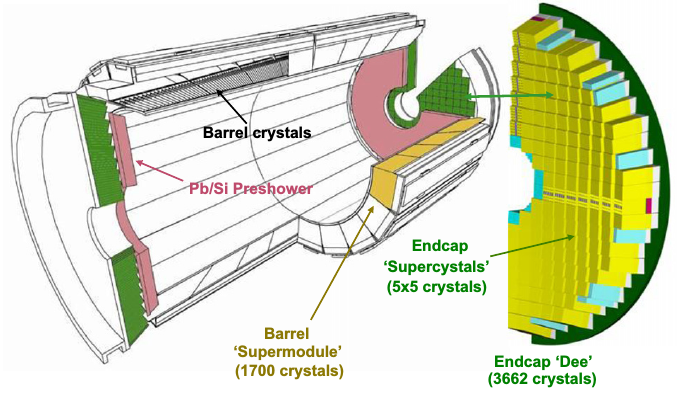
\includegraphics[height= 0.5\textwidth, width=0.7\textwidth]{THESISPLOTS/CMS-ECAL-EB-EE.png}}
%\mbox{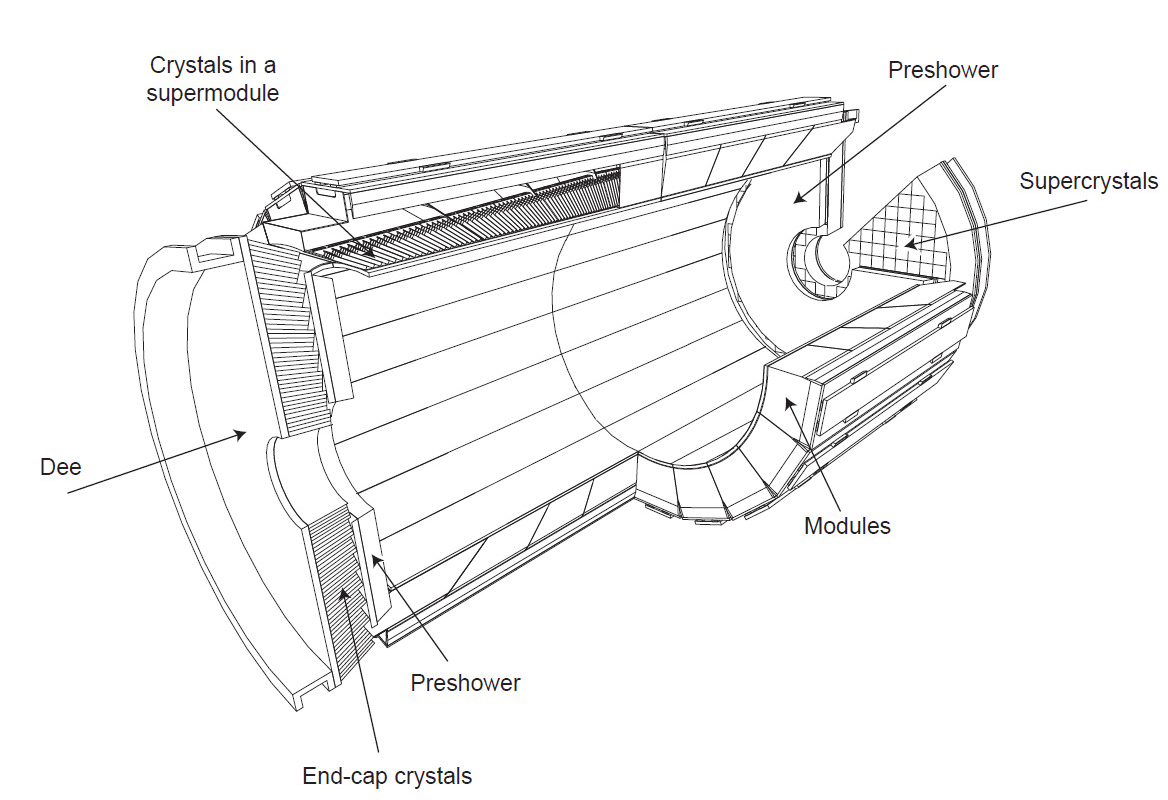
\includegraphics[scale=0.2]{THESISPLOTS/CMS-ECAL.png}}
%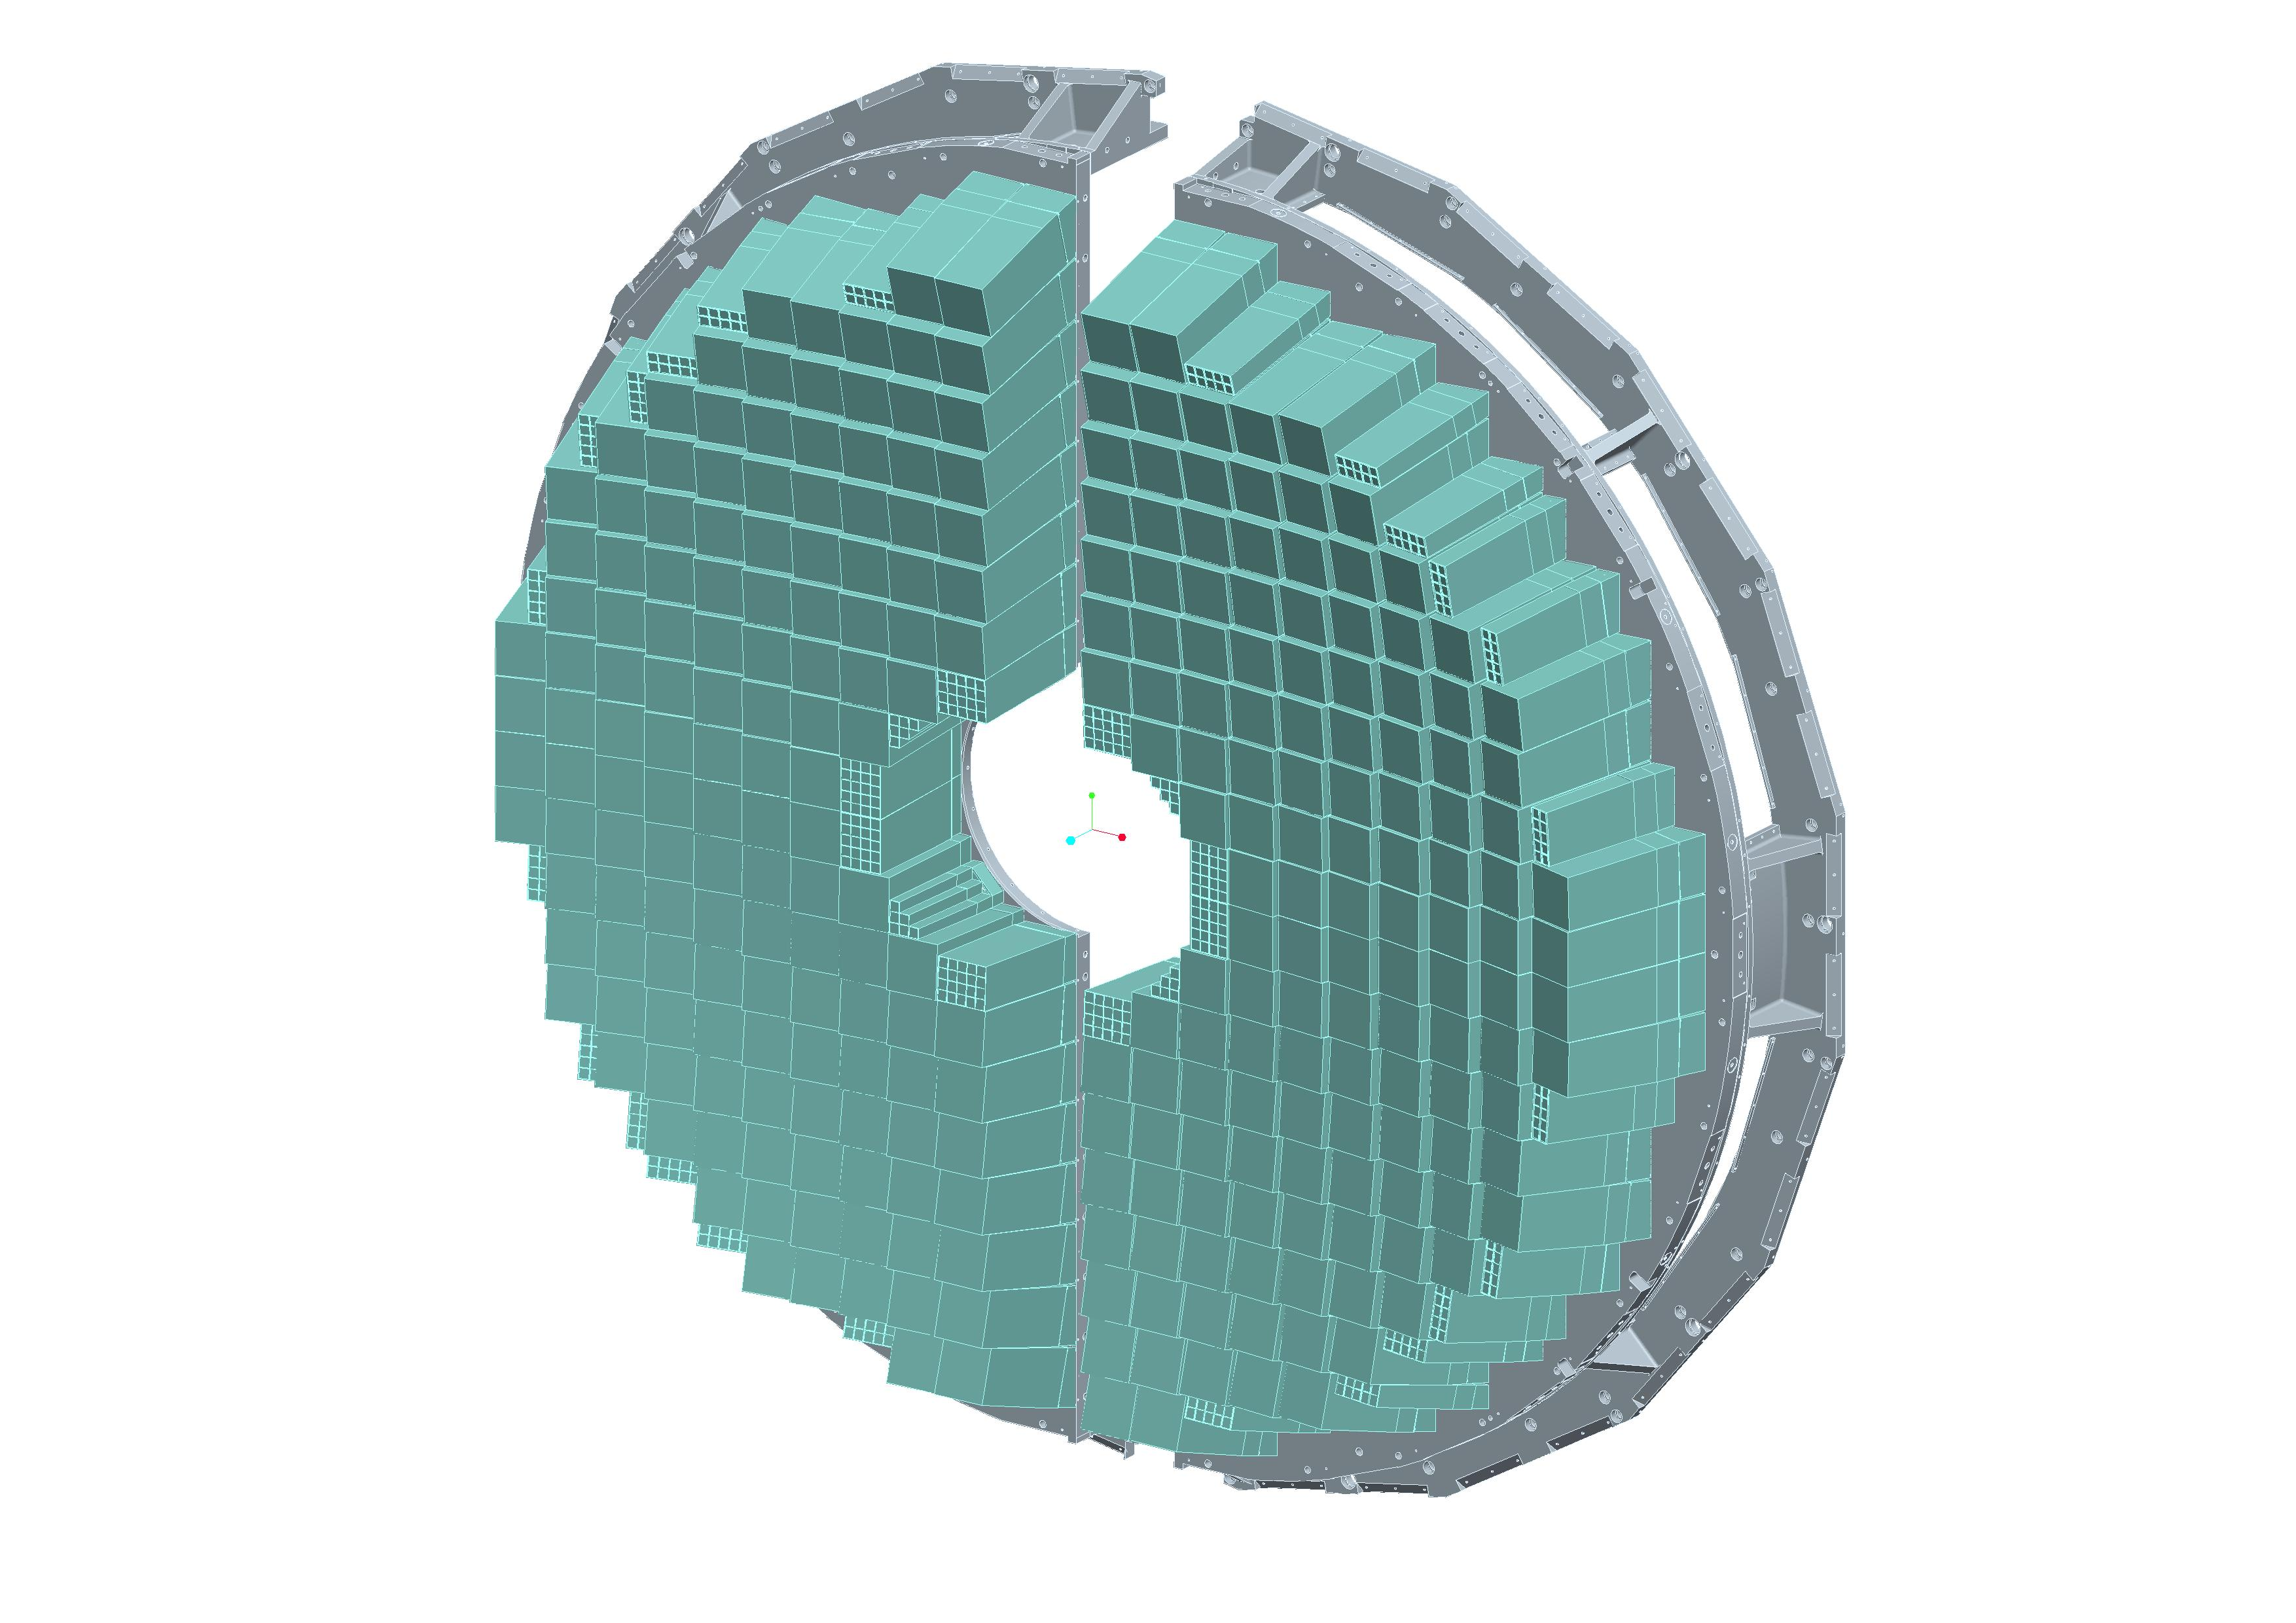
\includegraphics[scale=0.06]{THESISPLOTS/endcap_CMS.png}} 
\captionof{figure}{Layout of the CMS electromagnetic calorimeter showing the arrangement of crystal modules, supermodules in the barrel with the preshower infront of endcap with supercrystals.}
\label{fig:CMSECAL}
\end{center}

%%%%%%%%%%%%%%%%%%%%%%%%%%%%%%%%%%%%%%%%%%%%%%%%%%%%%%%%%%%%%%%%%%%%%
\begin{center}\label{CMS-SUBD}
\centering
\mbox{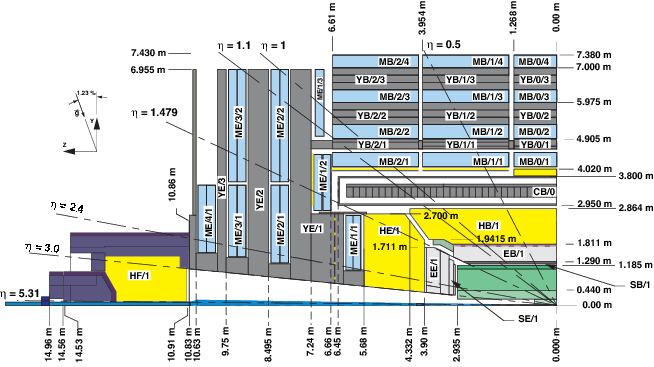
\includegraphics[height= 0.5\textwidth, width=0.7\textwidth]{THESISPLOTS/CMS_Int_View.png}} 
\captionof{figure}{Cross section view showing the coverage range of CMS sub-detectors and their longitudinal distance from the IP.}
\label{fig:cmslview}
\end{center}
\clearpage
%\subsection{Particle Detection}
%Particle types that are identified using the CMS detector include electrons, photons, hadrons, muons, neutrinos and other weakly interacting particles. These particles depending on their charge, nature of interaction and lifetime can be identified either using some or all the sub-detectors of the CMS detector.
%The figure \ref{fig:cmsSLICE} show a  transverse slice of the CMS detectors with tracks in the tracker and muon sub-detectors and calorimeter energy deposit showing how different particles interact with the material in different sub-detectors thus ensuring their unique identification and reconstruction in the detector.
%\begin{center}
%\centering
%\mbox{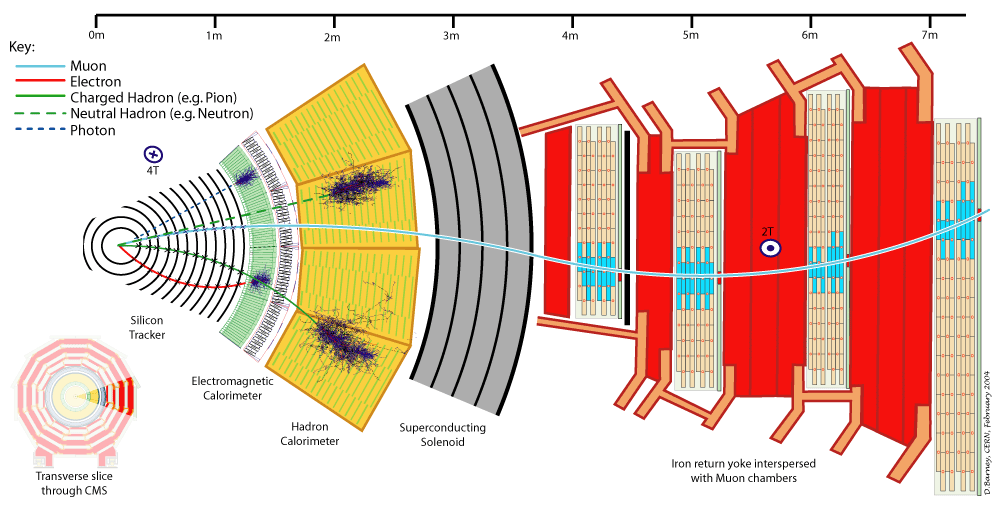
\includegraphics[scale=0.4]{THESISPLOTS/CMS_Slice.png}} 
%\captionof{figure}{Transverse slice of the CMS detector showing how different types of particles interact and hence identified using this detector.}
%\label{fig:cmsSLICE}
%\end{center}
\subsection{Triggering}
In CMS, there are a billion interactions including \textit{pile up}~(PU) happening each second. This means data from each 25~ns proton-proton collision has to be processed and stored before the next collision happens. Also, since not all these collisions produce 
interesting physics events, we have to be capable of selecting only interesting physics events produced from proton-proton collisions with sufficient  energy. The process of selecting such interesting events is called \textit{triggering}.
%Even with this selection, it is not possible to process a single event in a 25~ns time frame. Thus, the 
CMS uses a two level triggering system for selecting interesting events produced with enough energy from collisions.
The comprise of the \textit{Level}-1~(L1) and \textit{High Level Triggers}~(HLT) triggers.
% with enough energy. and a pipeline system to temporarily store and process information from many interactions at the same time. The pipeline system helps to separate events belonging to different bunch crossings~(BX).
%Signals from millions of electronic channels from subdetectors are identified and synchronized  produced by the same event.
%The \textit{Level}-1~(L1) and \textit{High Level Triggers}~(HLT) triggers make up the CMS triggering system.
\newline
The L1 triggers is a hardware designed electronics system implemented in FPGA and ASIC technology and uses information from the calorimeter, muon trigger and a global trigger board. The global trigger board makes the final decision based on the calorimeter and muon triggers to reject or keep an event for further processing at the HLT trigger. The L1 trigger is responsible for selecting the best 100,000 events/second from the initial 1 billions events/second produced. %The pipeline system is used during the L1 trigger latency time of about 3.2~$\mu$s.
\newline
The HLT is a software comprised of implemented selection algorithms running on a farm of more than 1000 standard computers. %Thus event selection begins at the L1 and HLT triggers.. 
These complex algorithms include instructions like, match tracks to hits from the muon chambers, select energy deposits above a certain threshold in the calorimeters with no tracks for electromagnetic objects, and begins the first step of event selection. Just like the L1 trigger, the HLT  uses assimilated and synchronized information from different parts of the CMS detector to create the entire event. 
By the time this selection process is complete, there are now only 100 events/second with the remaining 99,900 thrown away.
Taking an average event size to be 1~Megabyte, in a stable and effective LHC proton collision period of a year or $10^{7}$~seconds, CMS produces about a Petabyte of data which is stored and used later for offline physics analysis.
% Due to the large amount of data, such analysis are performed using clusters of computers geographically connected to each other in a virtual computing environment called the LHC Computing Grid~(LCG) to which the CMS is a member. This data is made available to 7 primary and later to secondary tier centres consisting of national research laboratories and universities around the world using a data transport system term Physics Experiment Data Export~(PhEDEx).
\label{Collider_And_Detector_chapter}
%%%%%%%%%%%%%%%%%%%%%%%%%%%%%%%%%%%%%%%%%%%%%%%%%%%%%%%%%%%%%%%%%%%%%%%%%%%%%%%%
